\documentclass[DM,lsstdraft,authoryear,toc]{lsstdoc}
% lsstdoc documentation: https://lsst-texmf.lsst.io/lsstdoc.html

% Package imports go here.
\usepackage{graphicx}
\usepackage{url}
\usepackage{latexsym}
\usepackage{color}
\usepackage{enumitem}

% Local commands go here.

% To add a short-form title:
% \title[Short title]{Title}
\title[Alerts Menu]{LSST Alerts: Science-Driven Options for Packets and their Distribution}

% Optional subtitle
% \setDocSubtitle{A subtitle}

\author{%
M.~L.~Graham and the Data Management System Science Team, with contributions from the Transients and Variable Stars Science Collaboration
}

\setDocRef{DMTN-TBD}
\date{\today}
% Optional: name of the document's curator
% \setDocCurator{The Curator of this Document}
\setDocUpstreamLocation{\url{https://github.com/lsst-dm/dmtn-xxx}}

\setDocAbstract{%
\textcolor{red}{\bf EXTREME DRAFT STATE. DO NOT CITE. DO NOT READ. LOOK AWAY.}\\
A review and discussion of the variety of options for alert packets and their distribution, such as latency timescale, packet contents, pre-stream filtering, and so forth.
}

% Change history defined here.
% Order: oldest first.
% Fields: VERSION, DATE, DESCRIPTION, OWNER NAME.
% See LPM-51 for version number policy.
\setDocChangeRecord{%
  \addtohist{0}{2019-11-14}{Conception.}{Melissa Graham}
  \addtohist{0.1}{2020-01-09}{First draft ready for input from others.}{Melissa Graham}
}

\begin{document}

% Cite requirements using these macros.
% \lsrreq \ossreq \dmreq \reqparam 

% Create the title page.
% Table of contents is added automatically with the "toc" class option.
\maketitle

% % % % % % % % % % % % % % % % % % % % % % % % % %
\section{Introduction} \label{sec:intro}

% The LSST Science Requirements Document \citedsp{LPM-17} specifies that information about the detections of transient, variable, and moving objects be released promptly as a data stream.

The purpose of this document is to consider the science motivation for, and impact of, various options for alert packet contents and their distribution timescale.
The contents and delivery of alert packets will play a major role in the scientific impact of LSST, in part because they are the only LSST data product that is both world public, as they are exempt from any proprietary period, and publicly accessible because they are distributed to community brokers, and not solely available via the LSST Science Platform (LSP).
In comparison, although the contents of the Prompt products database (PPDB) from which alerts are generated are also world public, access to the PPDB is restricted to individuals with data rights \citedsp{LDO-013} who have authenticated accounts in the LSP.

It is a requirement\reqparam{numStreams}\dmreq{0391} that the DMS be capable of supporting the transmission of at least 5 full alert streams within 60 seconds of image readout.
This is based in part on estimates of the alert stream data rate and the bandwidth allocated to alert distribution in the LSST data facility.
Reducing the packet size or increasing (slightly) the latency could enable the stream to be delivered to more brokers, and thereby increase the amount of alerts-related science done by the community.
The alert packets, as described in \citeds{LSE-163}, were designed to include all the relevant LSST data about a source that a broker might need to assess, classify, and prioritize the alert for follow-up observations \emph{within minutes} (i.e., on order the timescale of the 60 second alert distribution latency).
Reducing the contents should only be done if that information is easily and quickly obtainable elsewhere. 

{\bf Document Overview ---} \S~\ref{sec:packets} discusses how removing stamps and histories from alerts could be scientifically beneficial for some brokers, as long as stamps are made publicly available with similar latency, and proposes additional alert elements to better identify potential transient host galaxies.
\S~\ref{sec:latency} find that most alerts-related science goals would be satisfied with a $\sim$5 minute alert timescale, but that the quickly evolving fields of fast radio bursts and gravitational wave events may soon provide more robust motivation for a 60 second latency.
\S~\ref{sec:prefilter} lists types of pre-filtered streams that could improve brokers' scientific productivity and estimates the resulting bandwidth reductions, and \S~\ref{sec:graceful} argues that when alerts are delayed, the scientifically optimal response would be to flag and distribute them as soon as possible (and not, e.g., send them directly to an archive).

%This draft contains content pertaining to the following open tickets in the DM-SST epic "Studies Around Alerts" (assignees):
%\begin{itemize}
%\item DM-19484, Estimate distribution of alert packet size based on scientific considerations (Bellm)
%\item DM-15654, Define policy for handling fields with $>$10K alerts (Bellm)
%\item DM-20296, Investigate the possibility of providing filtered streams (Graham)
%\item DM-20298, Revise the contents of the alert packets (Graham)
%\item DM-20299, Scientific use-cases requiring $<$5 minute access (Graham)
%\item DM-20300, Investigate options for expanding access to the alert stream (Bellm)
%\end{itemize}

\clearpage
% % % % % % % % % % % % % % % % % % % % % % % % % %
\section{Alert Packet Contents} \label{sec:packets}

In this section the scientific impacts of various options to reduce the size of alert packets (in order to, e.g., enable wider alert distribution, facilitate broker processing) are considered, as are potential additions to the alert packet contents which would improve the user's ability to classify and prioritize alert sources for follow-up.
The main conclusions of the following discussion are:
\begin{itemize}
\item {\bf Removing Histories (\S~\ref{sssec:packets_remove_hist}) ---} Removing the {\tt DIASource} histories from the alert packets that are transmitted to brokers that request this modification could be scientifically beneficial, but a list of all {\tt DIASource} identifiers associated with the {\tt DIAObject} at the time of alert generation must be added to those packets. 
\item {\bf Removing Stamps (\S~\ref{sssec:packets_remove_stamps}) ---} Removing the image stamps from all alert packets could be scientifically beneficial, but stamps should still be made during alert production and made publicly retrievable with a latency similar to that of alert distribution.
\item {\bf Distributing Multiple Packet Formats (\S~\ref{sssec:packets_remove_procon}) ---} From a science perspective, distributing non-identical alert packets would have no negative impact provided that full-sized packets do not become more prone to delays.
\item {\bf Adding Object Association Information (\S~\ref{ssec:packets_add}) ---} To better enable extragalactic transient science with brokers, two new {\tt DIAObject} catalog elements should be computed and included in the alert packets: (1) the {\tt objectId} for the three {\tt Object} catalog galaxies with the lowest separation distance (based on the galaxy's 2D luminosity profile) from the {\tt DIAObject}, and (2) the separation distances for those three {\tt Objects}.
\item {\bf Compressing Packets (\S~\ref{ssec:packets_compress}) ---} From a science perspective, compressing the alert packets has little scientific impact unless it imposes a large additional latency on alert distribution, which could be detrimental to alerts-related science.
\end{itemize}

\subsection{Removing Histories and/or Stamps}\label{ssec:packets_remove}

The size of a fully-loaded individual alert packet is estimated to be $\lesssim$82~KB, based on simulations of the planned content of the alerts as described in Section 3.5 of \citeds{LSE-163} (see also \citeds{DMTN-102}).
The two largest components of the alert packet which could be considered ``optional'' are the history and the postage stamps.
The history is the past $\sim$12 months of {\tt DIASource} records, previously released as alerts.
The postage stamps are, at minimum, 30$\times$30 pixels and contain flux, variance, and mask extensions for both the template and difference image, plus a header of metadata \citedsp{LSE-163}.
The history accounts for $\sim$27KB of the alert packet ($\sim$33\%) and the stamps contribute $\gtrsim$18~KB ($\sim$20\%). 

Brokers that save all alerts, build their own a database of alerts contents, or have an automated interface with the LSST Prompt products database or Alerts database might not need the historical records to be included in the alert packets.
Brokers which do not use the image stamps -- or would need them for only a subset of the alerts and could feasibly query a stamps database -- might not need them included in the alerts packets.
Individual broker teams may indicate which information they require (or would like removed from the packets in their stream) during the broker proposal process \citedsp{LDM-612,LDM-682,LDM-723}.
During the first stages of the proposal process, and at the LSST Community Brokers Workshop\footnote{\url{ls.st/cbw}} in June 2019, there was some indication that at least a few brokers were interested in alerts without historical records and/or postage historical records.

\subsubsection{{\tt DIASource} Record History}\label{sssec:packets_remove_hist}

Including the {\tt DIASource} record history in every alert allows for the \emph{instant assessment} --- without the need to cross-match or query catalogs --- of changes in the objects's location, size, shape, or brightness, provides context for the latest detection (i.e., anomalous or typical), and enables a robust assessment of the likely physical nature of the object (e.g., light curve fits indicating supernova type become more reliable with more observations). 

To remove the {\tt DIASource} record history from an alert would slightly inhibit the scientific assessment of transient/variable objects for brokers that build their own database of alert contents, due to the time required to cross-match with the database.
Removing the {\tt DIASource} record history would completely inhibit this kind of analysis for brokers that do not have such storage or processing capabilities.

There is also the issue that the association of {\tt DIASources} into {\tt DIAObjects} may change over time, for some objects.
For example, rare cases such as multiply-imaged strongly-lensed supernovae, or two unassociated transients/variables that are superimposed along the line of sight, might be blended/separated in poor/good seeing.
In such cases, the set of all associated {\tt DIASources} might be improved between one alert and the next. 

{\bf Summary --} The {\tt DIASource} record histories should not be removed from all alert packets, but could be optionally removed at the request of a broker.
However, if the record histories are removed, a list of all {\tt DIASource} identifiers (the {\tt diaSourceId}, as in Section 3.3.1 of \citeds{LSE-163}) which are currently associated with the {\tt DIAObject} to which the alert-spawning {\tt DIASource} is associated should be provided (note that this list is \emph{not} currently part of the {\tt DIAObject} record).

\subsubsection{Forced Photometry History}\label{sssec:packets_remove_fp}

When forced photometry ({\tt DIAForcedSource} record history) is included in an alert packet, it is ``historical" in the sense that it is based on past images and not the image which spawned the alert.
However, it is not always redundant information that was previously released in an alert, like the {\tt DIASource} record history.

There are two main cases where forced photometry is performed, as described in \citeds{LSE-163}.
(1) For all new {\tt DIAObjects}, forced ``pre-covery'' photometry is done in the past 30 days of difference images within 24 hours, stored in the {\tt DIAForcedSource} catalog, and included in all future alert packets associated with that {\tt DIAObject}.
(2) For all {\tt DIAObjects} that are not detected\footnote{The detection threshold is a signal-to-noise ratio $\geq$ 5.} in a given difference image, but had a detection in the past $\sim$12 months, forced photometry is done on that difference image.
The result is stored in the {\tt DIAForcedSource} catalog, and included in all future alert packets associated with that {\tt DIAObject}.
The forced photometry is scientifically valuable because, for example, pre-covery forced photometry provides context for the first detection of a transient/variable, and low-SNR detections can help with photometric classification and prioritization for follow-up observations. 

If a given {\tt DIAObject} is never again detected in a difference image, then the {\tt DIAForceSource} records are never included in an alert packet, but are available to individuals or brokers with access to the PPDB via the LSST Science Platform.
If a given {\tt DIAObject} is repeatedly detected in new difference images, then the same {\tt DIAForcedSource} records will be redundantly included in all future alerts (after the first one containing the pre-covery or non-detection forced photometry).
For the ``historical" {\tt DIAForcedSource} records, alert content redundancy could be avoided by only including previously undistributed {\tt DIAForcedSource} data in an alert packet.
To do this, the Prompt pipeline would have to either compare with the contents of the most recent alert and remove redundant data from the new alert, or flag the {\tt DIAForcedSource} data as ``released" and only add ``unreleased" forced photometry to a alert packet.
Both of these options would add processing times to the alert generation pipeline, which is undesirable.

{\bf Summary --} If the decision is made to remove the historical {\tt DIASource} records from alert packets, the {\tt DIAForcedSource} records of forced photometry should always be added to all alerts.
This will cause some redundancy in alert contents, but if not included there would be no public access to this scientifically valuable information.

\subsubsection{Postage Stamps}\label{sssec:packets_remove_stamps}

\textcolor{red}{MLG notes from DESC: not all alerts need them so it could be, e.g., for new DIASources only, non-stellar DIASources, etc. with the rest going to a server that does not have the 1 minute latency requirements.}

Including the postage stamps in the alert packet allows for the instant assessment of the {\tt DIASource} in the difference and template images, which has a variety of scientific applications.
For example, although real/bogus classification of the difference-image sources will be done prior to alert generation, some brokers may still wish to run additional algorithms on the images -- especially in the case of first detections.
Brokers might also employ algorithms to classify transients and variables based on the images instead of the photometry (e.g., \citealt{2019PASP..131j8006C}).
From the postage stamp images, scientifically useful information can be derived about the trails left by moving objects, or from the 2-dimensional luminosity distribution of spatially evolving objects such as comets, which might not be entirely captured by the {\tt DIASource} elements (see Table 1 in \citeds{LSE-163}).
The images also provide context for the {\tt DIASource}, such as host-galaxy morphology or field crowdedness, that can assist with follow-up observations.

If postage stamps were not created during alert production, the only option would be for users to wait until the images are made available (within 24 hours) in the LSP, which would significantly inhibit alerts-based science goals.
However, postage stamps are unlikely to be needed for most {\tt DIASources}, the majority of which --- 95\%, according to the breakdown in \citeds{DMTN-102} --- will be stars or asteroids: point sources for which context is not a significant part of their immediate evaluation.
An efficient compromise might be for the Prompt pipeline to create the postage stamps during alert generation, and then store them in a publicly accessible database (i.e., outside the LSP) where they can be obtained (via {\tt diaSourceId}) with a latency similar to the alert distribution timescale by anyone, from anywhere, at anytime. 

The expected maximum download rate from this stamp database is estimated by assuming that all 5 community brokers download $\sim$500 stamp sets per visit: $\sim$2500 stamp sets every $\sim$35 seconds.
At 18~KB per stamp set, that's a data rate of 10.5 Mbps (for comparison, that's $\sim$5\% of one full alert stream).

{\bf Summary --} The postage stamps could be removed from all alert packets, but they should still be created during Prompt processing and stored in a publicly accessible database where they can be obtained with a latency similar to the alert distribution timescale.

\textcolor{red}{{\bf Could Postage Stamps Be Smaller? --}}
\citeds{LSE-163} describes the size of the postage stamp to be at least $6\arcsec \times 6\arcsec$ ($30\times30$ pixels), or large enough to encompass the entire footprint of the {\tt DIASource} (e.g., if trailed, extended). 
That is large enough to contain the angular diameter (30 kpc) of a Milky Way-like galaxy at a redshift of $z\approx0.5$, which will be a fairly typical supernova host galaxy in the LSST data set.
Since context is a science driver for producing stamps, it would not be desirable for them to be much smaller than $6\arcsec \times 6\arcsec$.


\subsubsection{Pros and Cons of Multiple Alert Formats}\label{sssec:packets_remove_procon}

The histories and/or stamps could be removed from all alert packets, or only at the request of a broker.
In the latter case, LSST might end up distributing four types of alert packet formats to its five brokers: (i) with histories and stamps, (ii) with histories but without stamps, (iii) without histories but with stamps, and (iv) without histories or stamps. 

From a science perspective, the benefits to allowing brokers to customize their alert packet is that it potentially enables unique science to be done by brokers (e.g., very rapid custom stamp-analysis algorithms), and could enable LSST to support $>$5 brokers which might lead to more alerts-related science in general.

One drawback might arise during times of heavy load, such as many visits with $>$40,000 alerts (\S~\ref{sec:graceful}), \emph{if}, and only if, full-sized packet streams are more likely to be delayed.
Whether this becomes a possibility will depend on the technical aspects of how the multiple types of alerts are generated and transmitted, and also on the final decisions about latency (\S~\ref{sec:latency}) and delayed distribution (\S~\ref{sec:graceful}).
This may well never come to pass, but if it did, it could be unfair to brokers requiring full-size packets.
While some brokers are being designed for a wide variety of science goals, others are more specifically tailored.
If it is the specifically-tailored broker that requires full-sized alerts, then experiencing delayed transmission more frequently than other brokers could put some science goals at a disadvantage. 
Furthermore, the fact that not all alert packets are identical might cause some additional bookkeeping considerations for downstream brokers who ingest from multiple community brokers, but that should not be detrimental to their science goals.
The technical considerations of how many different alert packet formats it is feasible to create and transmit within the required latency time is beyond the scope of this document, in which we focus on science impacts.

{\bf Summary --} Offering multiple alert formats to brokers is scientifically beneficial provided that full-sized alerts are not predisposed to delay.

\subsection{Additional {\tt Object} Association Information}\label{ssec:packets_add}

\textcolor{red}{MLG notes from DESC: \\ (1) Check "Host Galaxy Identification for Supernova Surveys" \citet{2016AJ....152..154G}. \\ (2) Alex Gagliano is working on host association as a part of classification that does a PCA on galaxy properties, and found that color and morphology are the first two PCA components, and that the hosts of SNIa SNII etc. occupy different parts of the PC2 vs PC1 plane. His paper is in prep still. \\ (3) As MWV was trying to tell you, host association depends on the redshift of the object (i.e., you want to do it in absolute distance); obviously that won't be in the alert so we can't make it part of the "3 nearest", but you'll probably want to mention that specifically.}.

The contents of the alert packet as defined in \citeds{LSE-163} includes the following with respect to associations with {\tt Object} catalog from the most recent data release:
\begin{itemize}
\item {\tt nearbyObj} ({\tt unit64[6]}), the {\it "closest {\tt Objects} (3 stars and 3 galaxies) in Data Release database"}
\item {\tt nearbyObjDist} ({\tt float[6]}), the {\it "distances to {\tt nearbyObj}"} in arcseconds
\item {\tt nearbyObjLnP} ({\tt float[6]}), the {\it "natural log of the probability that the observed {\tt DIAObject} is the same as the nearby {\tt Object}"}
\end{itemize}
For the latter, there is a footnote that says {\it "This quantity will be computed by marginalizing over the product of position and proper motion error ellipses of the {\tt Object} and {\tt DIAObject}, assuming an appropriate prior"}.

The current definitions of {\tt nearbyObj}, {\tt nearbyObjDist}, and {\tt nearbyObjLnP} are not as useful as they could be for transients in host galaxies. 
For extragalactic transients, the three nearest galaxies are not always the three most likely host galaxies, and the distance in arcseconds matters less than a separation distance that accounts for the galaxy's luminosity profile.
Furthermore, the definition of {\tt nearbyObjLnP} is only appropriate for static variable point sources (stars): for transients in host galaxies, the observed {\tt DIAObject} will never be ``the same as the nearby {\tt Object}".

Statistically, the most likely host for a given transient is the galaxy which contributes the most optical flux at the transient's location.
This is usually estimated by calculating an offset distance from the nearby galaxies to the transient that is expressed in terms of the galaxy's spatial luminosity profile, and assuming the galaxy with the lowest offset distance is the host.
The following are several options for estimating which nearby galaxy is the most likely host of an extragalactic transient.

{\bf Effective Radius --} Calculate a separation distance that is the radial distance from the core of the galaxy to the location of the transient, divided by the effective radius of the galaxy (i.e., {\tt kronRad90} in the {\tt Objects} table; \citeds{LSE-163}).
The nearby galaxy with the lowest separation distance is the most likely host. This will account for the relative sizes of the potential host galaxies, but not their position angles. 

{\bf Second Moment --} Calculate a separation distance, as in \citet{2006ApJ...648..868S}, based on the two-dimensional luminosity profile of the galaxy.
Where $x_{\rm trans},y_{\rm trans}$ is the location of the transient, and $x_{\rm gal},y_{\rm gal}$ is the center of the galaxy (the first moment; {\tt radec} in the {\tt Object} table), the separation distance is $R^2 = C_{xx} x_r^2 + C_{yy} y_r^2 + C_{xy} x_r y_r$, where $x_r = x_{\rm SN} - x_{\rm gal}$ and $y_r = y_{\rm SN} - y_{\rm gal}$.
The ellipse parameters $C_{xx}$, $C_{yy}$, and $C_{xy}$ can be calculated directly from the second moments of the galaxy luminosity profile ({\tt Ixx}, {\tt Iyy}, and {\tt Ixy} in the {\tt Object} table), e.g., as described in Section 10 of E. Bertin's Source Extractor manual\footnote{Version 2.3: \url{https://www.astromatic.net/pubsvn/software/sextractor/trunk/doc/sextractor.pdf}}.
The nearby galaxy with the lowest separation distance is the most likely host.
This option accounts for both the relative sizes and position angles of the potential host galaxies, and requires only a little more processing. 

{\bf 2D Algorithms --} There are also other, more complicated methods for identifying the most likely host for a given transient.
For example, the nearby galaxy with the smallest fraction of light interior to an isophot through the transient's location, where the isophot shape is given more degrees of freedom and not constrained to concentric ellipticals as in the second moment method above.
Another example is to use an algorithm that provides deblended footprints for nearby extended objects, and can estimate the fraction of light in given pixel that should be attributed to each (e.g., the SCARLET deblender, \cite{2018A&C....24..129M}).
\textcolor{red}{\citeds{LSE-163} does mention that footprints will be generated for {\tt Objects}, but it doesn't look like they'd be stored in the {\tt Object} table; find out if these footprints would be appropriate/available to use here.}
The most likely host galaxy would be the one which contributes the most flux at the pixel location of a transient.

Generally, nearby galaxies with separation distances $>$3, or $>$99\% of the luminosity profile, are not assigned as hosts and the transient is considered "hostless".
While this cutoff has been appropriate for past samples of $\sim$hundreds of transients, it will not be appropriate for the LSST sample size, and no such cut should be applied when evaluating potential host galaxies for {\tt DIAObjects}. 

All of the above host galaxy identification methods can also make use of priors if the transient type is known; for example, the established correlation between core-collapse supernovae and star formation.
However, such a robust level of host associations are beyond scope for the Prompt pipeline, and the main goal is to provide brokers with sufficient information to assess the potential host association, and decide whether it is useful to the classification and/or prioritization of alerts for follow-up. 

{\bf Summary --} For the ten nearest {\tt Object} catalog galaxies, a separation distance should be calculated with respect to the transient location, preferably using the second moments of each galaxy's luminosity profile. Two new {\tt DIAObject} catalog elements should be added: {\tt nearbyPotHost}, containing the {\tt objectId} for the three galaxies with the lowest separation distances, and {\tt nearbyPotHostSepDist}, containing the separation distances. An analog for the existing element {\tt nearbyObjLnP}, representing the probability, is not necessary. This would add {\tt unit64[3]} and {\tt float[3]} to the {\tt DIAObject} catalog and to each alert, but this both tiny and worthwhile.

\subsection{Compressing the Alert Packets}\label{ssec:packets_compress}

The application of gzip compression could further reduce the size of a full alert to $\sim$65~KB (80\%; JIRA ticket DM-16280).
Naively, this seems like it would allow 1 more full stream to be transmitted to a broker, and thereby enable more science.
However, the time and computational resources required to compress the alert packets needs to be considered.
For example, gzip compression at 50 MB/s to compress $\sim$10000 alerts would take $\sim$10000 $\times$0.08 MB per alert $/$50 MB/s, or $\sim$16 seconds.
This is significant, considering the alert distribution latency requirement\reqparam{OTT1}\lsrreq{0101}\ossreq{0127}\dmreq{0004} is 60 seconds. 
Furthermore, compressing the alert packets forces brokers to then decompress the alerts on arrival, which would incur further delay.
Science goals requiring very low-latency alerts distribution might be negatively impacted by compression -- see \S~\ref{sec:latency} for a deeper discussion of the science drivers for low-latency alerts.

{\bf Summary --} Since packet compression could induce an additional latency, perhaps it should only be done if, e.g., an algorithm could provide a compression rate of $\lesssim$10 MB/s (requiring only a few seconds to compress a visit's worth of alerts), or if the alert distribution latency requirement is relaxed from 1 minute (see \S~\ref{sec:latency}).
Otherwise, compression would have no impact on alerts-related science goals and so this should be primarily a technically-driven decision.




\clearpage
% % % % % % % % % % % % % % % % % % % % % % % % % %
\section{Alert Distribution Latency} \label{sec:latency}

This section considers the scientific motivation for the 1 minute alert distribution latency, and the impact to alerts-related science if that latency was extended to, e.g., 5 minutes.
It is a requirement that the DMS be capable of supporting the distribution of at least 98\%\reqparam{OTT1}\reqparam{OTR1}\lsrreq{0101}\lsrreq{0025}\ossreq{0127}\dmreq{0004} of alerts for each visit within 60 seconds of the end of image readout.
However, if it is possible to relax this requirement without a negative impact on science then it might be possible for LSST to transmit alerts to $>$5 brokers (and/or repurpose human and computational resources dedicated to the 1 minute latency), which in turn might enable more alerts-related science.

Generally, for science goals that require alerts on timescales shorter than $\sim$5 minutes, this need stems from targets that are fast-evolving or short-lived (or both) and require follow-up on timescales shorter than $\sim$15--30 minutes.
Since most observing strategies for the WFD main survey do not revisit fields on timescales shorter than $\sim$15 minutes (strategies that do pair visits aim for closer to $\sim$22 minute gaps), brokers must be able to confidently identify such targets with single-epoch single-filter LSST photometry, or be using additional information (e.g., host galaxy characteristics, coincident alerts from other surveys).
For the purposes of this discussion, an optimistic outlook is assumed, and the difficulty in identifying targets with a single epoch of LSST photometry is not considered as a reason to downgrade the importance of a 1 minute alert latency.

After a consideration of the following science cases that are most likely to require rapid follow-up (summary below), it appears that most of them would be satisfied without risk if the latency was increased from 1 to 5 minutes. 
However, it is absolutely not unambiguously clear that a need for 1 minute alerts will not evolve out of the still emergent fields of fast radio bursts and gravitational wave events over the next couple of years.
\begin{itemize}
\item {\bf A TVS Survey (\S~\ref{ssec:latency_tvs})} found that only $<$10\% of respondents reported that requiring alerts within 1 minute was necessary for their science goals.
\item {\bf GW Follow-up (\S~\ref{ssec:latency_emgw}) ---} Although a 5 minute latency would suffice for kilonovae (days-long optical counterparts to neutron star mergers), some theoretical models predict optical emission within the first hour (e.g., jet break-out or spin-down energy from the merger). However, these GW scientific motivators for a 1 minute alert latency are moot if the time between GW event and LSST ToO follow-up remains at tens of minutes or more.
\item {\bf Gamma-Ray Bursts (\S~\ref{ssec:latency_grb}) ---} \textcolor{red}{Tentatively,} alerts for the coincident optical counterparts of short GRBs would be most scientifically useful if distributed within 1 minute, but the predicted occurrence rate is $\lesssim$20 over the 10-year LSST survey.
\item {\bf Fast Radio Bursts (\S~\ref{ssec:latency_frb}) ---} \textcolor{red}{Tentatively,} some models predict that a short, bright burst of optical emission from the physical mechanism powering FRBs could be detected by LSST 5 to 15 minutes prior to the radio signal.
If such optical events occur with significant frequency, are bright and consistently detectable, and can be identified with a single-filter detection, and if radio telescopes can respond within minutes, then LSST is the most promising future facility for this science, which requires a 1 minute alert distribution latency.
\item {\bf Young Supernovae (\S~\ref{ssec:latency_ysne}) ---} The science goals require follow-up in an hour or longer, and a 5 minute latency would not have a negatively impact.
\item {\bf Solar System Objects (\S~\ref{ssec:latency_sso}) ---} \textcolor{red}{TBD.}
\item {\bf Stellar Variables (\S~\ref{ssec:latency_stars}) ---} \textcolor{red}{TBD.}
\end{itemize}


\subsection{TVS Survey Results Regarding Alerts Timescales}\label{ssec:latency_tvs}
{\it Contents contain the results of a TVS survey administered by Rachel Street.}

The Transients and Variable Stars (TVS) science collaboration surveyed the science needs of their members with respect to alert latency, and the results\footnote{Results courtesy of TVS co-chair Rachel Street.} are shown in Table \ref{tab:tvs}.
The survey asked respondents to choose the maximum tolerable and ideal average delay between the alerts being produced by the LSST data reduction pipeline and the alert information becoming available through the broker service.
This is not exactly the same as the alert distribution timescale {\tt OTT1}, but these responses will inform the need for $<$1 minute alert distribution.
Respondents were asked to provide a short summary of their science goals for alerts if they reported needed access within 15 minutes.
Note that the pool of respondents is probably not representative of the wider collaboration, and is likely biased towards individuals with science interests that do require faster access to alerts. 

\begin{table}[h]%[htdp]
\caption{Table of results from a TVS survey which asked "how fast do you really need alerts?". The total number of respondents was 20. The science driver acronyms are: EM-GW (electromagnetic counterparts to gravitational wave events), YSNe (young supernovae, including e.g., shock breakouts), GRBs (gamma-ray bursts). \label{tab:tvs}}
\begin{center}
\begin{tabular}{|l|cl|cl|}
\hline
             & Maximum & Science & Ideal       & Science \\
Latency & Tolerable  & Driver(s) &  Average & Driver(s) \\
\hline
1 min or less & 1 & EM-GW, GRB  & 2 & EM-GW, YSNe, GRB \\
1-5 min         & 0 &                          & 1 &                                   \\
5-10 min       & 1 & EM-GW, YSNe & 1 & YSNe \\
10-30 min     & 2 & YSNe               & 2 & EM-GW, GRBs \\
30-60 min     & 2 &                          & 7 & EM-GW  \\
1-6 hours     & 4 & EM-GW, GRBs & 1 &  \\
6-12 hours   & 2 &                          & 1 &  \\
12-24 hours & 3 & EM-GW            & 1 & EM-GW \\
1-3 days      & 1 &                           & 0 &  \\
>3 days       & 4 &                           & 4 &  \\
\hline
\end{tabular}
\end{center}
\label{default}
\end{table}%

Only 20\% (10\%) of respondents report that $<$10 minutes ($\leq$1 minute) is an ideal average delay, and whereas 70\% report that $>$30 minutes would be a sufficient average latency.
The three science drivers associated with $<$5 minute alert access are the electromagnetic counterparts to gravitational wave events (EM-GW; kilonovae), young supernovae (early short-lived light curve features such as shock breakouts), and gamma-ray bursts (GRB).
The fact that these three are also listed as science drivers for longer-latency alert is mainly due to the diversity within the science drivers and the fact that the events have both short- and longer-timescale features.
Each of these science drivers is discussed in turn below, along with two other science cases that rely on rapid access to LSST alerts: fast radio bursts (FRBs) and solar system objects (SSOs).

\subsection{EM Counterparts to GW Events}\label{ssec:latency_emgw}
{\it Some contents revised from a Slack conversation between Federica Bianco, Om Sharan Salafia, and Eric Bellm.} \textcolor{red}{MLG notes from DESC: the case for optical counterparts to neutrino events falls in this category as well, with perhaps the same challenge of them being not instantaneous so there is already some $>10$ minute delay such that 60s optical alerts from any follow-up aren't the bottleneck.}

During LSST Operations, target-of-opportunity imaging follow-up sequences might be executed in the error ellipse of a gravitational wave (GW) detection to search for the electromagnetic (EM) optical counterpart.
Such a search yielded a fast-evolving "kilonova" which decayed from 22 to 28th magnitude in the $g$-band in just 6 days \citep[faster in the bluer and slower in the redder filters][]{2017Sci...358.1559K}.
Although the kilonova light curves last only a few days, since there is so far only one event, GW170817, a day or two delay between the GW event and the optical detection still yields very scientifically valuable data -- for now.
During LSST Operations there will already exist a sizable collection of longer-latency follow-up, and it is likely that science will be moving in the direction of pushing to ever earlier detections.
However, since kilonovae produce days-long optical afterglows, a 5 minute LSST alerts would likely suffice.

There are two theoretical predictions for prompt optical emission that would require very rapid access to alerts.
One of them is a potential faint, $<$1 hour, UV/optical transient that occurs at the time of jet-break out for a short gamma-ray burst associated with a binary neutron star merger (\S~\ref{ssec:latency_grb}).
Another that predicts emission of a similar color, luminosity, and timescale is the spin-down energy of a long-lived ($10^2$--$10^4$ s) neutron star formed from a binary neutron star merger before its eventual collapse to a black hole \citep{2016ApJ...819...15S}.
As described in \S~\ref{ssec:latency_grb}, very few events could be detected by serendipitous coincidence by the LSST WFD main survey, and targeted follow-up of well-localized GW events with more appropriate facilities such as space-based UV/optical imagers is much more likely to yield detections of this very short lived emission.

There are two additional issues related to ToO for EMGW events which might make 1 minute alerts necessary or impossible. 

First, for rapid ToO observations when visit coordinates are not known in advance, there might not be time to pre-cache the slow database queries that are needed during alert production processing (e.g., loading slices of the PPDB catalogs).
This might mean that an alert distribution latency cannot be guaranteed for ToO imaging surveys. 
For the purposes of this science-driven discussion, assume this to be a surmountable technical implementation issue.

The second is that, at least for run O3, the GW event detection system itself issues preliminary alerts within 1--10 minutes, and these preliminary alerts are often retracted and do not always have the sky localization.
Even now, many imaging follow-up surveys wait for the initial alert (or retraction) to be sent after a round of human vetting of the GW event signal, and this can take several hours.
With such latencies, the question of 1 {\it vs.} 5 minute LSST alert timescales becomes inconsequential. 

\subsection{Gamma-Ray Bursts}\label{ssec:latency_grb}

{\it \textcolor{red}{MLG: no outside input on this yet, is needed to be confirmed by a GRB person.} }

\citet{2018ApJ...854L..13H} searched for fast-fading transients in archival data from the intermediate Palomar Transient Factory (iPTF) and found 50 candidates, three of which were confirmed to be the afterglows of long GRBs. Of these three, two were in the archival data because the iPTF had done dedicated follow-up observations of Fermi detections, and one was serendipitous. They estimate an all-sky rate of such optical transients (peak $m<18$ mag, fade by at least 2 mag in 3 hours) of $680^{+2236}_{-119}$ events per year (similar to that of long GRBs). \textcolor{red}{MLG: still need some LSST projection here.}

Short gamma-ray bursts (sGRBs) are thought to be the mergers of two neutron stars, or a neutron star and a black hole.
As the jet propagates through the ejecta material a hot cocoon is formed.
When cocoon and jet break out, along with the sGRB can be observed a blue optical transient with an absolute peak brightness of -12 to -15 magnitudes which lasts for $10^3$--$10^4$ seconds (e.g., \citealt{2018MNRAS.473..576G}).
For an LSST detection limit of $r\sim24$ mag, a detection limit of $r\lesssim-12$ ($r\lesssim-15$) mag corresponds to distances of $\lesssim160$ ($\lesssim630$) Mpc, or redshifts $z\lesssim0.035$ ($z\lesssim0.14$).
Observing the diversity of cocoon emission for a sample of sGRBs would require regular and consistent multi-band follow-up within $10^3$ seconds, or $15$ minutes.
In such cases where a sGRB is observed in a time/area that is serendipitously coincident LSST visit, science would be maximized if the alert confirming the presence of an optical counterpart was distributed to brokers within 1 minute.
However, what is the expected frequency of this situation occurring during LSST Operations?

% z=0.035 is V=0.014 Gpc3
% z=0.14 is V=0.836 Gpc3
% (0.836/0.014) * 4/yr = 240/yr
The rate of short GRBs in the local volume ($<$200 Mpc) is estimated to be quite low, $<$4 $\rm yr^{-1}$ \citep{2019arXiv190800100M}.
Scaled up to the co-moving volume within 630 Mpc, this rate is $\sim$240 $\rm yr^{-1}$, all-sky.
In the baseline main survey about a sixth of the sky can be observed in a given night, which implies $\sim$1 sGRBs with detectable optical counterparts in the WFD survey per night for every $\sim$10 nights of observations.
The probability that one of the 1000 visits per night will occur during the 5 minutes in which an alert would be useful for triggering rapid follow-up is $<10^{-2}$.
Very roughly, we might expect this serendipitous coincidence to occur twice a year at most, or $\sim$20 times over the 10-year LSST main survey.

% 10 visits per 5 minute block, or 100 "blocks" per night
% 100x100 potential sky area/time options for the 100 blocks, x10 days
% of the options, 100 blocks per night x 10 nights would be done
% and then randomly draw just the 1 sGRB
% scipy.stats.hypergeom(100000,1000,1)
% 0 0.9900 
% 1 0.0100 
% 2 0.0000 

For discovering the optical counterparts of sGRBs, the LSST wide-fast-deep survey is simply not the most efficient future facility for the job.
As described by \citet{2018MNRAS.473..576G}, a rapid search at the location of sGRBs with a UV satellite such as ULTRASAT would be ideal.

%Triggering criteria might be:
%new {\it u}- or {\it g}-band source with recent limits associated with a $<$200 Mpc galaxy (how many expected per night?)
%and then very high priority if it's serendipidously associated with a GRB detection in the last 5 minutes

\subsection{Fast Radio Bursts}\label{ssec:latency_frb}

{\it Some contents based on text from and discussions with Tyler Pritchard.}

One of the most likely -- but also most mysterious -- transients that might significantly benefit from the $60$ second alert timescale are fast radio bursts (FRBs): a millisecond long pulse of coherent emission in the GHz range.
The emission is dispersed by the inter-galactic medium (IGM), such that the pulse's observed arrival time is frequency dependent.
Observed FRB dispersion measures of $\rm{DM}\approx100$ to $1000$ $\rm pc\ cm^{-3}$ indicate that they originate at cosmological distances, with redshifts $z\approx0.1$ to $1$ \citep{2018Natur.562..386S}. 

If an optical counterpart is generated by this coherent emission, the time delay between the optical detection and the radio detection is on the timescale of minutes for frequencies $\nu < 500\ {\rm MHz}$, as shown in Figure \ref{fig:sci_frb}.
This leaves open the possibility for triggering radio follow-up of an optical counterpart candidate serendipitously detected by LSST -- if such counterparts exist and are detectable.
A millisecond-long event in the optical would have to be quite bright to be detected by LSST, but studies show that LSST detections are feasible \citep{2016ApJ...824L..18L}.
\cite{2019ApJ...878...89Y} demonstrate that two theoretical sources for coherent optical emission from FRBs would not be detectable by LSST, but that inverse Compton scattering processes could lead to optical detections with LSST (e.g., from pulsars or masers).
Searches for FRB counterparts in optical images that were serendipitously obtained (near-) coincidentally with an FRB detection have only just recently become possible thanks to current wide-field imaging surveys.
No transient optical counterparts have yet been detected \citep{2019ApJ...881...30T}, but individual host galaxies for FRB events have been identified \citep{2016Natur.530..453K}.

Since the rate of FRBs is estimated to be quite high (thousands per day; \citealt{2016MNRAS.460L..30C}) even after radio detection efficiency is factored in there could be many within the observed LSST volume. 
For example, if there are 1000 FRB occurring across the full sky every 24 hours, and LSST observes one sixth of the sky during a night's 10 hours of darkness, then there would be $\sim70$ FRB occurring in that area during that time.
Assuming that both the FRB and the LSST visits are distributed randomly in time and location (although the visits are correlated, obviously), there's a $\sim6\%$ chance that in any given night one visit will be serendipitously coincident with the expected arrival of a short lived optical precursor to the FRB.
If such a source could be recognized as an FRB optical counterpart within a minute, and radio follow-up could begin as soon as possible to detect the radio component and measure the time delay (Figure \ref{fig:sci_frb}).  
However, \textcolor{red}{it is (or rather, MLG is) currently unclear whether (a) there is strong theoretical support for such optical counterparts, and (b) radio telescopes can perform ToO follow-up on $<$15 minute timescales}.

If FRBs are associated with superluminous supernovae (SLSNe) and young magnetars, then potentially an LSST alert regarding a change in behavior of known SLSNe could be used to trigger radio follow-up.
However, this case is unlikely to be as sensitive to the LSST alert distribution timescale as the optical emission would be released over a longer time window \citep{2019arXiv191002036L}.

\begin{figure}[h]
\begin{center}
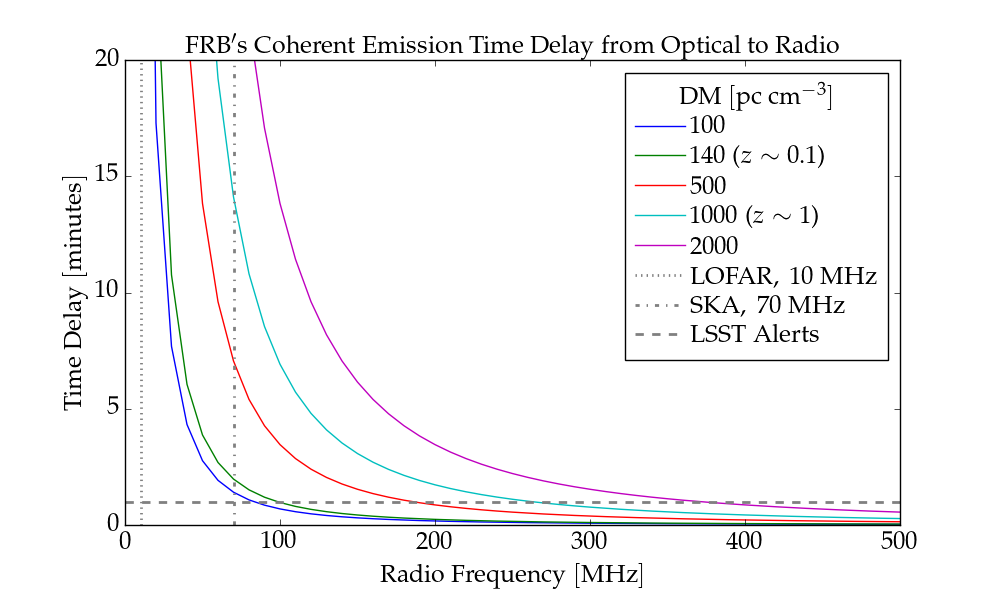
\includegraphics[width=15cm]{figures/frb_optical_delays.png}
\caption{The delay time (for coherent emission) between the arrival of the optical and radio photons due to cosmological dispersion, as a function of the frequency of the radio detector. The {\it lowest} frequency bands of the Square Kilometer Array (SKA) and the Low-Frequency Array (LOFAR) are marked with vertical dotted and dash-dotted lines, and the 1 minute timescale for LSST alert distribution with a horizontal dashed line. The delay time is $\Delta t = k_{\rm DM}\,DM\,(\nu_{\rm low}^{-2} - \nu_{\rm high}^{-2})$, where $k_{DM}=4.149$ $\rm GHz^2\ pc^{-1}\ cm^3\ ms$, ${\rm DM}$ is the dispersion measure in $\rm pc\ cm^{-3}$, $\nu$ is the low and high frequency bands of the observation, and $\Delta t$ is in $\rm ms$. We have used the range of FRB dispersion measures as observed by \cite{2018Natur.562..386S}. \label{fig:sci_frb}}
\end{center}
\end{figure}

\subsection{Young Supernovae}\label{ssec:latency_ysne}

Photometric data obtained during the first few hours to days of a supernova can constrain the progenitor radius and circumstellar material in the immediate environment, which in turn provides information about the progenitor star, its system, and its final stages of evolution before the explosion.
For example, \citet{2018Natur.554..497B} model the optical photometric data of the post-shock breakout cooling peak for a massive star's core collapse supernova to constrain the radius and mass of its outer envelope; \citet{2012ApJ...744L..17B} used the first day of photometric observations of a nearby Type Ia (thermonuclear detonation) supernova to show that their progenitor stars must be a compact degenerates; and rare ``blue bumps" in the first few days of a Type Ia supernova's light curve might betray the presence of a non-degenerate companion star \citep[e.g.,][]{2010ApJ...708.1025K,2017ApJ...845L..11H}.

For young supernovae, follow-up observations within a couple of hours are required, and the related science goals are unlikely to be impacted if the alert latency was 5--10 minutes instead of 1 minute.

\subsection{Solar System Objects}\label{ssec:latency_sso}

\textcolor{red}{MLG: in Lynne's talk on the SSSC needs for alerts brokers at the CBW in June 2019, slide 4 says that a needed broker capability was "API or other 'push' notification (e.g., trailed detections) [minutes may count]". Follow-up on the SS use case for alerts on very short timescales.}

\subsection{Stellar Variables}\label{ssec:latency_stars}

\textcolor{red}{Return to the road map or science book? Surely there must be some stellar use-cases for 1 minute alerts. E.g., microlensing peaks can be real sharp.}

\citet{2006ApJ...644L..63K}, the discovery of three $<$hour optical transients in the Deep Lens Survey (one confirmed M star and two with potentially extragalactic origin), has been invoked as motivation for the 30 second exposure times and 60 second alert production latency -- e.g., the Deep Lens Survey is referenced without citation in the LSST Science Requirements Document. More recently, \citet{2013ApJ...779...18B} searched for fast optical transients in the Pan-STARRS1 Medium-Deep Survey identified 19 fast transients: 11 M dwarf flares and 8 likely solor system objects. \citet{2018ApJ...854L..13H} searched for fast-fading transients in archival data from the Palomar Transient Factor and found 50 candidates: three GRB afterglows (\S~\ref{ssec:latency_grb}), eight artifacts, one asteroid, and 38 with red stellar counterparts identified as M dwarfs. \textcolor{red}{Their Fig 1 is a delta-mag vs. delta-time plot comparing afterglows to Mdwarf flares that shows how they can be photometrically distinguished (difference regions of that parameter space)}. \textcolor{red}{Existence of short duration M dwarf flares established; what's the science related to them?}



\clearpage
% % % % % % % % % % % % % % % % % % % % % % % % % %
\section{Pre-Filtered Alert Streams} \label{sec:prefilter}

This section explores the scientific motivation and impact of offering brokers pre-filtered alert streams. 
Pre-filtering could reduce the overall bandwidth of alert distribution and potentially allow streams to be transmitted to more brokers, thereby enabling more alerts-related science.
Providing pre-filtered streams could also lessen the load and resources used by the brokers, enabling more alerts-related science by allowing brokers to spend a smaller fraction of their budget computational resources.

Depending on the science goals of a given broker and/or their users, a broker might find it useful to only receive alerts for {\tt DIASources} which:
\begin{itemize}
\item are likely to have a certain physical origin, e.g., stellar variable, moving objects
\item could potentially be observed by the follow-up resources its users have access to
\item have at least one prior detection by LSST (because, e.g., their algorithms all require photometric confirmation or a change in brightness)
\item originate in images obtained as part of a special program such as the deep drilling fields or target-of-opportunity imaging surveys
\item were not obtained during poor weather conditions (e.g., an image quality or sky background violating some limit)
\end{itemize}

For the above science drivers, the types of pre-filters that are likely to be scientifically useful -- some of which have been suggested by brokers already -- include:
\begin{itemize}
\item {\bf Apparent Magnitude:} only {\tt DIASources} brighter than a specified apparent magnitude (for each of the LSST filters {\it ugrizy}) are transmitted. 
\item {\bf Region of Sky:} only {\tt DIASources} in a given sky area (or areas; defined by, e.g., limits in right ascension or declination), are transmitted. 
\item \texttt{\bf DIAObject} {\bf History:} only {\tt DIASources} associated with {\tt DIAObjects} that have at least $N$ previous detections are transmitted, where $N$ can be $\geq1$. 
\item \texttt{\bf SSObject} {\bf Association:} only {\tt DIASources} that are associated with a {\tt SSObject} are transmitted. (Potentially including new, unassociated {\tt DIASources}, because they might also be moving objects).
\item \texttt{\bf Object} {\bf Association:} only {\tt DIASources} associated with {\tt DIAObjects} that are, in turn, associated with a data release {\tt Object} that meets some specification are transmitted (e.g., associated with a stellar point source).
\item {\bf Observation Metadata:} only alerts from images obtained with a given set of metadata, e.g., a special observing program or meeting sky condition thresholds, are transmitted.
\end{itemize}

All of these potential science-driven pre-filters are based on the information contained in the alert itself, and do not impose any additional processing on the Prompt pipeline.
They all also have the potential to considerably reduce the number of transmitted alerts.
Due to the exponential relationship between the number of variable stars and their variability amplitude, and also that of volume and distance modulus, an apparent magnitude limit $\sim1$ mag brighter than the nominal $5{\sigma}$ {\tt DIASource} detection limit could reduce the alert stream data rate by $\gtrsim50$\%.
Limiting to alerts that are associated with past detections or certain types of objects could similarly reduce the alert stream data rate.
These types of pre-filers would reduce the number of alerts per visit for all visits -- the average bandwidth -- which might enable alert distribution to extend to more brokers and thus enable more alerts-related LSST science.
Pre-filters based on their sky location or observational metadata would probably either deliver all or none of the alerts for a given visit, causing fluctuations in the bandwidth but not necessarily in a way that would allow for additional streams to be transmitted.


% % % % % % % % % % % % % % % % % % % % % % % % % %
\subsection{LSST Alert Filtering Service}\label{ssec:prefilter_lafs}

As described in \citeds{LSE-163} the LSST will provide an alert filtering service with limited capacity, by which individuals with LSST data rights and access may receive alerts via pre-defined filters and/or create and apply their own filters to the stream \citedsp{LPM-17,LSE-61}.
It is a requirement that the LSST alert filtering service be able to support\reqparam{numBrokerUsers}\dmreq{0343} at least 100 simultaneous users, and capable of returning 20\reqparam{numBrokerAlerts}\dmreq{0343} full-sized alerts per visit per user.
User-generated filters may be comprised of, e.g., a series of {\tt if} statements applied to the alert packet elements.
There are no requirements on the latency of filter execution, which may depend on the complexity of the filter and available resources. 

From a science perspective, it would be beneficial to offer any and all of the pre-filtered streams listed above as options for user-generated filters.
Individual users running small follow-up programs are more likely to have access to smaller-aperture telescopes and thus desire an initial apparent magnitude cut.
It would save on compute resources to avoid a situation in which, e.g., 50 user-generated brokers all start with an {\tt if} statement to filter the stream to, e.g., $m_r < 20$ mag. 

% One type of simple filtering that individual users are more likely to want than brokers is ``watchlist" capability -- lists of individual objects (stars or galaxies) and offset radii that alerts are desired within. 





\clearpage
% % % % % % % % % % % % % % % % % % % % % % % % % %
\section{Graceful Degradation} \label{sec:graceful}

The LSST specifications for the DMS require that it support the distribution\reqparam{transN}\lsrreq{0101}\reqparam{nAlertVisitAvg}\ossreq{0193}\reqparam{nAlertVisitPeak}\dmreq{0393} of at least 40,000 alerts per single standard visit, and that for visits producing $\leq$40,000 alerts \reqparam{sciVisitAlertDelay}\reqparam{sciVisitAlertFailure}\ossreq{0112}\dmreq{0392} no more than 1\% of them fail to have at least 98\% of its alerts distributed within 60 seconds of image readout.
It is furthermore specified that alert distribution "degrade gracefully" beyond that limit, meaning that visits resulting in an excess of 40,000 of alerts should not cause any DMS downtime \citedsp{LSE-30,LSE-61}.

This leaves the open question of what, from a science perspective, is the optimal way of dealing with delayed alerts that also meets the DMS specification of a ``graceful degradation"?
We leave the aspects of technical implementation of a ``graceful degradation", such as distributing delayed alerts and alert archive storage access, for elsewhere and here just consider the science implications for a delayed timescale.

{\bf Next-opportunity distribution via the alert stream.} As discussed in Section \ref{sec:latency}, there remains plenty of science goals that do not absolutely require alert distribution in 1 minute.
Distributing delayed alerts via the stream would still enable plenty of science.
The brokers might prefer to have delayed alerts clearly flagged to properly process them (e.g., some filtering and processing done by brokers might only be appropriate for alerts delivered within a given latency).

{\bf Next-morning distribution via the alert stream.} This refers to an option to collect all delayed alerts during the night and then releasing them (perhaps on a new ``topic") in the morning after survey operations have ended for the night.
From a science perspective this is not as useful as next-opportunity distribution, but if it is preferred for technical reasons it would enable more science than the option below.

{\bf Do not distribute delayed alerts; send directly to archive.} There is no scientific merit in not distributing delayed alerts, and two further drawbacks: the alert archive update timescale is 24 hours\reqparam{L1PublicT}, significantly slower than next-morning distribution, and the alert archive might only be accessible by brokers with data rights since it is part of the LSST Data Facility.

% MLG: commented out technical implementation aspects.
%The retention period of alert packets in the alert distribution system is still to be determined, but given the alert stream data rate of ~800 GB/night it is currently reasonable to expect a retention period of ~7 days. 
% It is a requirement that all alerts be stored in an archival database and be available for retrieval\ossreq{0185}.
%The term ``available for retrieval" applies to users with data rights and access to the LSST Science Platform.
%Like all other Prompt data products, the alerts archive will be updated within 24\reqparam{L1PublicT}\lsrreq{0104} hours \citedsp{LSE-29}.
% However, note that the requirements on user access to the alerts archive are not yet fully developed, and may be limited in terms of how alert packets may be queried (e.g., alert ID), or by the bulk download capabilities.



% Include all the relevant bib files.
% https://lsst-texmf.lsst.io/lsstdoc.html#bibliographies
\bibliography{local,lsst,lsst-dm,refs_ads,refs,books}

\end{document}
